%\nocite{35c5a183}
%\nocite{8b5861fc}
%\nocite{00000001}
%%%
We present an axiomatic approach to homology theory of which an overview is, for example, given in \cite{35c5a183}, where also further references can be found. For a traditional approach on homology which also provides a good intuition see some standard textbooks like \cite{8b5861fc}.
\\
Let us begin developing the algebraic framework of homology - sometimes referred to as homological algebra. Remember that the abelian groups and the group homomorphisms constitute a category denoted $\mathbf{Ab}$. A \textbf{chain complex (of abelian groups)} is a pair $(C,\partial)$ consistig of a sequence $C := (C_{n})_{n\in\mathbb{Z}}$ of abelian groups $C_{n} \in \mathrm{ob}_{\mathbf{Ab}}$ together with a sequence $\partial := (\partial_{n})_{n\in\mathbb{Z}}$ of group homomorphisms
\begin{align*}
  \partial_{n}
  \in
  \mathrm{mor}_{\mathbf{Ab}}(C_{n},C_{n-1})
\end{align*}
such that\footnote{here $0$ is the function that constantly maps to the group identity element}
\begin{enumerate}
\item[(CC)]
$\partial_{n-1} \circ \partial_{n} = 0$\qquad for all $n \in \mathbb{Z}$
\end{enumerate}
Such a chain complex is often depicted by the following diagram
\begin{equation*}
\begin{tikzcd}[row sep=2.2em,column sep=2.6em]
  \ldots
  \ar{r}{\partial_{n+1}}
  &
  C_{n}
  \ar{r}{\partial_{n}}
  &
  C_{n-1}
  \ar{r}{\partial_{n-1}}
  &
  C_{n-2}
  \ar{r}{\partial_{n-2}}
  &
  \ldots
\end{tikzcd}
\end{equation*}
A \textbf{cochain complex (of abelian groups)} is a pair $(C^{\prime},\partial^{\prime})$ consisting of a sequence $C^{\prime} := (C^{n})_{n\in\mathbb{Z}}$ of abelian groups $C^{n} \in \mathrm{ob}_{\mathbf{Ab}}$ together with a sequence $\partial^{\prime} := (\partial^{n})_{n\in\mathbb{Z}}$ of group homomorphisms
\begin{align*}
  \partial^{n}
  \in
  \mathrm{mor}_{\mathbf{Ab}}(C^{n},C^{n+1})
\end{align*}  
such that
\begin{enumerate}
\item[(CC')]
$\partial^{n+1} \circ \partial^{n} = 0$\qquad for all $n \in \mathbb{Z}$
\end{enumerate}
often depicted as
\begin{equation*}
\begin{tikzcd}[row sep=2.2em,column sep=2.6em]
  \ldots
  &
  C^{n+2}
  \ar{l}[swap]{\partial^{n+2}}
  &
  C^{n+1}
  \ar{l}[swap]{\partial^{n+1}}
  &
  C^{n}
  \ar{l}[swap]{\partial^{n}}
  &
  \ldots
  \ar{l}[swap]{\partial^{n-1}}
\end{tikzcd}
\end{equation*}
From now on let $(C,\partial),(\hat{C},\hat{\partial}),(\tilde{C},\tilde{\partial})$ be chain complexes and $(C^{\prime},\partial^{\prime}),(\hat{C}^{\prime},\hat{\partial}^{\prime}),(\tilde{C}^{\prime},\tilde{\partial}^{\prime})$ be cochain complexes, where we often abuse notation by omitting the the sequence of homomorphisms, i.e. $C \doteq (C,\partial)$. A \textbf{chain map} is a sequence $f := (f_{n})_{n\in\mathbb{Z}}$ of group homomorphisms
\begin{align*}
  f_{n}
  \in
  \mathrm{mor}_{\mathbf{Ab}}(C_{n},\tilde{C}_{n})
\end{align*}
such that
\begin{enumerate}
\item[(CM)]
$\tilde{\partial}_{n} \circ f_{n} = f_{n-1} \circ \partial_{n}$\qquad for all $n \in \mathbb{Z}$
\end{enumerate}
It can be figured as the diagram
\begin{equation*}
\begin{tikzcd}[row sep=2.2em,column sep=2.6em]
  \ldots
  \ar{r}{\partial_{n+1}}
  &
  C_{n}
  \ar{r}{\partial_{n}}
  \ar{d}{f_{n}}
  &
  C_{n-1}
  \ar{r}{\partial_{n-1}}
  \ar{d}{f_{n-1}}
  &
  C_{n-2}
  \ar{r}{\partial_{n-2}}
  \ar{d}{f_{n-2}}
  &
  \ldots
  \\
  \ldots
  \ar{r}{\tilde{\partial}_{n+1}}
  &
  \tilde{C}_{n}
  \ar{r}{\tilde{\partial}_{n}}
  &
  \tilde{C}_{n-1}
  \ar{r}{\tilde{\partial}_{n-1}}
  &
  \tilde{C}_{n-2}
  \ar{r}{\tilde{\partial}_{n-2}}
  &
  \ldots
\end{tikzcd}
\end{equation*}
in which all the squares commute. Analogously, a \textbf{cochain map} is a sequence $f^{\prime} := (f^{n})_{n\in\mathbb{Z}}$ of group homomorphisms
\begin{align*}
  f^{n}
  \in
  \mathrm{mor}_{\mathbf{Ab}}(C^{n},\tilde{C}^{n})
\end{align*}
such that
\begin{enumerate}
\item[(CM')]
$\tilde{\partial}^{n} \circ f^{n} = f^{n+1} \circ \partial^{n}$\qquad for all $n \in \mathbb{Z}$
\end{enumerate}
depicted as the commuting diagram
\begin{equation*}
\begin{tikzcd}[row sep=2.2em,column sep=2.6em]
  \ldots
  &
  C^{n+2}
  \ar{d}{f_{n+2}}
  \ar{l}[swap]{\partial^{n+2}}
  &
  C^{n+1}
  \ar{d}{f_{n+1}}
  \ar{l}[swap]{\partial^{n+1}}
  &
  C^{n}
  \ar{d}{f_{n}}
  \ar{l}[swap]{\partial^{n}}
  &
  \ldots
  \ar{l}[swap]{\partial^{n-1}}
  \\
  \ldots
  &
  \tilde{C}^{n+2}
  \ar{l}[swap]{\tilde{\partial}^{n+2}}
  &
  \tilde{C}^{n+1}
  \ar{l}[swap]{\tilde{\partial}^{n+1}}
  &
  \tilde{C}^{n}
  \ar{l}[swap]{\tilde{\partial}^{n}}
  &
  \ldots
  \ar{l}[swap]{\tilde{\partial}^{n-1}}
\end{tikzcd}
\end{equation*}
The chain complexes are the objects of a category $\mathbf{CC}$ with chain maps as morphisms. Composition of chain maps $\hat{f} \in \mathrm{mor}_{\mathbf{CC}}(\hat{C},C)$ and $f \in \mathrm{mor}_{\mathbf{CC}}(C,\tilde{C})$ is given by composing the group homomorphisms for every $n \in \mathbb{Z}$ and can be figured by pasting diagrams together to obtain
\begin{equation*}
\begin{tikzcd}[row sep=2.2em,column sep=2.6em]
  \ldots
  \ar{r}{\hat{\partial}_{n+1}}
  &
  \hat{C}_{n}
  \ar{r}{\hat{\partial}_{n}}
  \ar{d}{\hat{f}_{n}}
  &
  \hat{C}_{n-1}
  \ar{r}{\hat{\partial}_{n-1}}
  \ar{d}{\hat{f}_{n-1}}
  &
  \hat{C}_{n-2}
  \ar{r}{\hat{\partial}_{n-2}}
  \ar{d}{\hat{f}_{n-2}}
  &
  \ldots
  \\
  \ldots
  \ar{r}{\partial_{n+1}}
  &
  C_{n}
  \ar{r}{\partial_{n}}
  \ar{d}{f_{n}}
  &
  C_{n-1}
  \ar{r}{\partial_{n-1}}
  \ar{d}{f_{n-1}}
  &
  C_{n-2}
  \ar{r}{\partial_{n-2}}
  \ar{d}{f_{n-2}}
  &
  \ldots
  \\
  \ldots
  \ar{r}{\tilde{\partial}_{n+1}}
  &
  \tilde{C}_{n}
  \ar{r}{\tilde{\partial}_{n}}
  &
  \tilde{C}_{n-1}
  \ar{r}{\tilde{\partial}_{n-1}}
  &
  \tilde{C}_{n-2}
  \ar{r}{\tilde{\partial}_{n-2}}
  &
  \ldots
\end{tikzcd}
\end{equation*}
Associativity and the identity morphisms are immediate from associativity and identities in $\mathbf{Ab}$. In the same fashion the cochain complexes and cochain maps constitute a category $\mathbf{CC^{\prime}}$.
\\
Now the condition (CC) for chain complexes is equivalent to say that
\begin{align*}
  \mathrm{im}(\partial_{n+1})
  &\subset
  \mathrm{ker}(\partial_{n})
  \qquad
  \text{for all }
  n
  \in
  \mathbb{Z}
\end{align*}
and the condition (CM) for chain maps implies that
\begin{align*}
  f_{n}
  \left(
    \mathrm{ker}(\partial_{n})
  \right)
  &\subset
  \mathrm{ker}(\tilde{\partial}_{n})
  \qquad
  \text{and}
  \qquad
  f_{n}
  \left(
    \mathrm{im}(\partial_{n+1})
  \right)
  \subset
  \mathrm{im}(\tilde{\partial}_{n+1})
  \qquad
  \text{for all }
  n
  \in
  \mathbb{Z}
\end{align*}
Hence the \textbf{$n$-th homology group}
\begin{align*}
  H_{n}(C)
  &:=
  \mathrm{ker}(\partial_{n})
  /
  \mathrm{im}(\partial_{n+1})
\end{align*}
is well-defined and so is the function\footnote{note that an element $[z] \in H_{n}(C)$ is represented by an element $z \in \mathrm{ker}(\partial_{n})$}
\begin{align*}
  H_{n}(f)
  \colon
  H_{n}(C)
  &\to
  H_{n}(\tilde{C})
  ,\quad
  [z]
  \mapsto
  [f_{n}(z)]
  \qquad
  \text{for }
  f
  \in
  \mathrm{mor}_{\mathbf{CC}}
  \left(
    C
    ,
    \tilde{C}
  \right)
\end{align*}
which in fact is a group homomorphism. An element of a homology group is often called \textbf{homology class} and two elements of the same homology class are called \textbf{homologous}. It is immediate that the $H_{n}$ are covariant functors from $\mathbf{CC}$ to $\mathbf{Ab}$ and we call them \textbf{homology group functors}. In a similar vein, using (CC') and (CM'), one defines the \textbf{$n$-th cohomology group}
\begin{align*}
  H^{n}(C^{\prime})
  &:=
  \mathrm{ker}(\partial^{n})
  /
  \mathrm{im}(\partial^{n-1})
\end{align*}
and group homomorphisms
\begin{align*}
  H^{n}(f^{\prime})
  \colon
  H^{n}(C^{\prime})
  &\to
  H_{n}(\tilde{C}^{\prime})
  ,\quad
  [z]
  \mapsto
  [f^{n}(z)]
  \qquad
  \text{for }
  f^{\prime}
  \in
  \mathrm{mor}_{\mathbf{CC^{\prime}}}
  \left(
    C^{\prime}
    ,
    \tilde{C}^{\prime}
  \right)
\end{align*}
yielding covariant functors $H^{n}$ from $\mathbf{CC^{\prime}}$ to $\mathbf{Ab}$ which we call \textbf{cohomology group functors}.
\\
Let us have a closer look at sequences of abelian groups. For this purpose let $I = \tilde{I} \cap \mathbb{Z}$ with $\tilde{I} \subset \mathbb{R}$ an interval. Then we call a sequence $(A_{n})_{n \in I}$ in $\mathrm{ob}_{\mathbf{Ab}}$ together with a sequence $(h_{n})_{n \land (n-1) \in I}$ of group homomorphisms
\begin{align*}
  h_{n}
  \in
  \mathrm{mor}_{\mathbf{Ab}}(A_{n},A_{n-1})
\end{align*}
\textbf{exact} if
\begin{align*}
  \mathrm{ker}(h_{n})
  &=
  \mathrm{im}(h_{n+1})
  \qquad
  \text{for }
  n
  \land
  (n-1)
  \land
  (n+1)
  \in
  I
\end{align*}
An \textbf{exact map} between exact sequences $(A_{n}) \doteq ((A_{n}),(h_{n}))$ and $(\tilde{A}_{n}) \doteq ((\tilde{A}_{n}),(\tilde{h}_{n}))$ with respect to $I$ is a sequence $(f_{n})_{n \in I}$ of group homomorphisms
\begin{align*}
  f_{n}
  \in
  \mathrm{mor}_{\mathbf{Ab}}(A_{n},\tilde{A}_{n})
\end{align*}
satisfying
\begin{enumerate}
\item[(EM)]
$\tilde{h}_{n} \circ f_{n} = f_{n-1} \circ h_{n}$\qquad for $n \land (n-1) \in I$
\end{enumerate}
If $I = \mathbb{Z}$ the exact sequence is called \textbf{long}. If $\mathrm{card}(I) = 5$ and the first group and the last group are trivial\footnote{we just write $0$ for the trivial group} the exact sequence is called \textbf{short}. Two short exact sequences and an exact map between them can thus be depicted as
\begin{equation*}
\begin{tikzcd}[row sep=2.2em,column sep=2.6em]
  0
  \ar{r}
  &
  \hat{A}
  \ar{r}{\hat{h}}
  \ar{d}{\hat{f}}
  &
  A
  \ar{r}{h}
  \ar{d}{f}
  &
  \tilde{A}
  \ar{r}
  \ar{d}{\tilde{f}}
  &
  0
  \\
  0
  \ar{r}
  &
  \hat{B}
  \ar{r}{\hat{g}}
  &
  B
  \ar{r}{g}
  &
  \tilde{B}
  \ar{r}
  &
  0
\end{tikzcd}
\end{equation*}
with commuting squares. The unique homomorphisms starting and ending at $0$ are omitted. Note that the exactness for a short sequence means that $\hat{h}$ is injective, $h$ is surjective and
\begin{align*}
  \mathrm{ker}(h)
  &=
  \mathrm{im}(\hat{h})
\end{align*}
Exact maps give rise to categories $\mathbf{LES}$ of long exact sequences and $\mathbf{SES}$ of short exact sequences, respectively. A short sequence
\begin{align*}
  \left(
    \left(
      0
      ,\hat{A}
      ,
      A
      ,
      \tilde{A}
      ,
      0
    \right)
    ,
    (0,\hat{h},h,0)
  \right)
  \in
  \mathrm{ob}_{\mathbf{SES}}
\end{align*}
is said to \textbf{split} if there is $r \in \mathrm{mor}_{\mathbf{Ab}}(\tilde{A},A)$ such that
\begin{align*}
  h
  \circ
  r
  &=
  \mathrm{id}_{\tilde{A}}
\end{align*}
One rather important statement is
\\
\begin{lem}[splitting lemma]
\label{lem:split}
For
\begin{align*}
  S
  &:=
  \left(
    \left(
      0
      ,
      \hat{A}
      ,
      A
      ,
      \tilde{A}
      ,
      0
    \right)
    ,
    (0,\hat{h},h,0)
  \right)
  \in
  \mathrm{ob}_{\mathbf{SES}}
\end{align*}
the following statements are equivalent:
\begin{enumerate}
\item[(i)]
there is $r \in \mathrm{mor}_{\mathbf{Ab}}(\tilde{A},A)$ such that
\begin{align*}
  h
  \circ
  r
  &=
  \mathrm{id}_{A}
\end{align*}
i.e. $S$ splits

\item[(ii)]
there is $l \in \mathrm{mor}_{\mathbf{Ab}}(A,\hat{A})$ such that
\begin{align*}
  l
  \circ
  \hat{h}
  &=
  \mathrm{id}_{\hat{A}}
\end{align*}

\item[(iii)]
$S$ is isomorphic to
\begin{align*}
  \left(
    \left(
      0
      ,
      \hat{A}
      ,
      \hat{A}
      \oplus
      \tilde{A}
      ,
      \tilde{A}
      ,
      0
    \right)
    ,
    (0,i,p,0)
  \right)
\end{align*}
where
\begin{align*}
  i
  \colon
  \hat{A}
  &\to
  \hat{A}
  \oplus
  \tilde{A}
  \qquad
  \text{and}
  \qquad
  p
  \colon
  \hat{A}
  \oplus
  \tilde{A}
  \to
  \tilde{A}
\end{align*}
are the inclusion and the projection, respectively.
\end{enumerate}
\end{lem}
Merging the concept of short exact sequences with the concept of chain complexes we get short exact sequences of chain complexes and a category $\mathbf{SES-CC}$ where exactness here means exactness for each $n \in \mathbb{Z}$. Let
\begin{equation*}
\begin{tikzcd}[row sep=2.2em,column sep=2.6em]
  0
  \ar{r}
  &
  (\hat{C},\hat{\partial})
  \ar{r}{\hat{f}}
  &
  (C,\partial)
  \ar{r}{f}
  &
  (\tilde{C},\tilde{\partial})
  \ar{r}
  &
  0
\end{tikzcd}
\end{equation*}
or more verbosely
\begin{equation*}
\begin{tikzcd}[row sep=2.2em,column sep=2.6em]
  &
  0
  \ar{d}
  &
  0
  \ar{d}
  &
  0
  \ar{d}
  &
  \\
  \ldots
  \ar{r}{\hat{\partial}_{n+2}}
  &
  \hat{C}_{n+1}
  \ar{r}{\hat{\partial}_{n+1}}
  \ar{d}{\hat{f}_{n+1}}
  &
  \hat{C}_{n}
  \ar{r}{\hat{\partial}_{n}}
  \ar{d}{\hat{f}_{n}}
  &
  \hat{C}_{n-1}
  \ar{r}{\hat{\partial}_{n-1}}
  \ar{d}{\hat{f}_{n-1}}
  &
  \ldots
  \\
  \ldots
  \ar{r}{\partial_{n+2}}
  &
  C_{n+1}
  \ar{r}{\partial_{n+1}}
  \ar{d}{f_{n+1}}
  &
  C_{n}
  \ar{r}{\partial_{n}}
  \ar{d}{f_{n}}
  &
  C_{n-1}
  \ar{r}{\partial_{n-1}}
  \ar{d}{f_{n-1}}
  &
  \ldots
  \\
  \ldots
  \ar{r}{\tilde{\partial}_{n+2}}
  &
  \tilde{C}_{n+1}
  \ar{r}{\tilde{\partial}_{n+1}}
  \ar{d}
  &
  \tilde{C}_{n}
  \ar{r}{\tilde{\partial}_{n}}
  \ar{d}
  &
  \tilde{C}_{n-1}
  \ar{r}{\tilde{\partial}_{n-1}}
  \ar{d}
  &
  \ldots
  \\
  &
  0
  &
  0
  &
  0
  &
\end{tikzcd}
\end{equation*}
be an object in $\mathbf{SES-CC}$. Note that $\hat{f}$ and $f$ are chain maps which means that all the squares commute. Then one can show that
\begin{align*}
  T_{n}
  \colon
  H_{n}(\tilde{C})
  &\to
  H_{n-1}(\hat{C})
  ,\quad
  [\tilde{z}]
  \mapsto
  \hat{f}_{n-1}^{-1}
  \left(
    \partial_{n}
    \left(
      f_{n}^{-1}([\tilde{z}])
    \right)
  \right)
\end{align*}
is well-defined for all $n \in \mathbb{Z}$. $(T_{n})$ is called \textbf{connecting homomorphism} since it {\glqq}connects{\grqq} an $n$-th with a $(n-1)$-st homology group. Here the maps $\hat{f}_{n-1}^{-1}$, $\partial_{n}$ and $f_{n}^{-1}$ are to be understood as the maps induced on the respective powersets when the homology classes are understood as subsets. One can further show that this connecting homomorphism yields a long exact sequence
\begin{equation*}
\begin{tikzcd}[row sep=2.2em,column sep=2.6em]
  \ldots
  \ar{r}
  &
  H_{n}(\hat{C})
  \ar{r}{H_{n}(\hat{f})}
  &
  H_{n}(C)
  \ar{r}{H_{n}(f)}
  &
  H_{n}(\tilde{C})
  \ar{r}{T_{n}}
  &
  H_{n-1}(\hat{C})
  \ar{r}
  &
  \ldots
\end{tikzcd}
\end{equation*}
Having all these basic notions introduced let us discuss the connection between homology and cohomology. In the following we assume $C_{n}$ to be a free group for all $n$. Further, let $G$ be an abelian group. Then taking
\begin{align*}
  C_{G}^{n}
  &:=
  \mathrm{mor}_{\mathbf{Ab}}(C_{n},G)
\end{align*}
together with
\begin{align*}
  \partial_{G}^{n}(\phi)
  &:=
  \phi
  \circ
  \partial_{n+1}
  \qquad
  \text{for }
  \phi
  \in
  C_{G}^{n}
\end{align*}
yields a cochain complex since
\begin{align*}
  \partial_{G}^{n+1}(\partial_{G}^{n}(\phi))
  &=
  \partial_{G}^{n+1}(\phi \circ \partial_{n+1})
  \\
  &=
  \phi
  \circ
  \partial_{n+1}
  \circ
  \partial_{n+2}
  \\
  &=
  \phi
  \circ
  0
  \\
  &=
  0
\end{align*}
One might call $C_{G}^{n}$ the dual abelian group of $C_{n}$ with respect to $G$ and $\partial_{G}^{n}$ - which is precomposition with $\partial_{n+1}$ - the dual homomorphism of $\partial_{n+1}$ with respect to $G$. So dualizing a chain complex results in a cochain complex just as it should be. One may now wonder if there also is a connection between homology groups and cohomology groups. And in fact, there is. It is stated in the universal coefficient theorem:
\\
\begin{thm}
\label{thm:uct}
If all $C_{n}$ in the chain complex $(C,\partial)$ are free and if $G$ is an abelian group then there is a short exact sequence of abelian groups
\begin{equation*}
\begin{tikzcd}[row sep=2.2em,column sep=2.6em]
  0
  \ar{r}
  &
  \mathrm{ext}(H_{n-1}(C),G)
  \ar{r}
  &
  H_{G}^{n}(C)
  \ar{r}
  &
  \mathrm{mor}_{\mathbf{Ab}}(H_{n}(C),G)
  \ar{r}
  &
  0
\end{tikzcd}
\end{equation*}
that splits.
\end{thm}
Here we have defined
\begin{align*}
  \mathrm{ext}(H_{n-1}(C),G)
  &:=
  \mathrm{mor}_{\mathbf{Ab}}(\mathrm{im}(\partial_{n}),G)
  /
  \mathrm{im}(i_{n-1}^{\prime})
\end{align*}
with
\begin{align*}
  i_{n-1}
  \colon
  \mathrm{im}(\partial_{n})
  &\to
  \mathrm{ker}(\partial_{n-1})
\end{align*}
the inclusion and
\begin{align*}
  i_{n-1}^{\prime}
  \colon
  \mathrm{mor}_{\mathbf{Ab}}(\mathrm{ker}(\partial_{n-1}),G)
  &\to
  \mathrm{mor}_{\mathbf{Ab}}(\mathrm{im}(\partial_{n}),G)
  ,\quad
  \phi
  \mapsto
  \phi
  \circ
  i_{n-1}
\end{align*}
its dual, which is nothing but the restriction to $\mathrm{im}(\partial_{n})$. The proof of theorem\footnote{it is actually worth to have a look at the proof, e.g. in \cite{8b5861fc}, because it can be done in a constructive manner and the definition of $\mathrm{ext}(H_{n-1}(C),G)$ becomes clearer then} \ref{thm:uct} shows that $\mathrm{ext}(H_{n-1}(C),G)$ is determined by $H_{n-1}(C)$ and $G$. Thus cohomology with respect to $G$ is determined by homology and $G$.
\\\\
We now turn to the more topological aspects of homology. For this purpose we define a category $\mathbf{Top_{2}}$ with objects the ordered pairs $(X,A)$ of toplogical spaces such that $A \subset X$ is a subspace and morphisms between pairs $(X_{1},A_{1})$, $(X_{2},A_{2})$ in $\mathrm{ob}_{\mathbf{Top}_{2}}$ the continuous maps
\begin{align*}
  f
  \colon
  X_{1}
  &\to
  X_{2}
  \quad
  \text{with}
  \quad
  f(A_{1})
  \subset
  A_{2}
\end{align*}
Moreover we define a functor $P \colon \mathbf{Top_{2}} \to \mathbf{Top_{2}}$ assigning to an object $(X,A)$ the object $(A,\emptyset)$ and assigning to a morphism $f \colon (X_{1},A_{1}) \to (X_{2},A_{2})$ its restriction to $A_{1}$. Then a \textbf{homology theory} is a sequence $(H_{n})_{n\in\mathbb{Z}}$ of covariant functors
\begin{align*}
  H_{n}
  \colon
  \mathbf{Top_{2}}
  &\to
  \mathbf{Ab}
\end{align*}
together with a sequence $(\mathsf{T}_{n})_{n\in\mathbb{Z}}$ of natural transformations
\begin{align*}
  \mathsf{T}_{n}
  \colon
  H_{n}
  &\to
  H_{n-1}
  \circ
  P
\end{align*}
which means that for $f \colon (X_{1},A_{1}) \to (X_{2},A_{2})$ the diagram
\begin{equation*}
\begin{tikzcd}[row sep=2.5em,column sep=3em]
  H_{n}((X_{1},A_{1}))
  \ar{r}{H_{n}(f)}
  \ar{d}[swap]{\mathsf{T}_{n}((X_{1},A_{1}))}
  &
  H_{n}((X_{2},A_{2}))
  \ar{d}{\mathsf{T}_{n}((X_{2},A_{2}))}
  \\
  H_{n-1}((A_{1},\emptyset))
  \ar{r}{H_{n-1}(P(f))}
  &
  H_{n-1}((A_{2},\emptyset))
\end{tikzcd}
\end{equation*}
commutes for all $n \in \mathbb{Z}$, such that
\begin{enumerate}
\item[(HT1)]
for all $(X,A),(Y,B) \in \mathrm{ob}_{\mathbf{Top_{2}}}$, if
\begin{align*}
  f_{0},f_{1}
  \colon
  (X,A)
  &\to
  (Y,B)
\end{align*}
are homotopic via a homotopy $(h_{s})_{s\in[0,1]}$ with $h_{s} \in \mathrm{mor}_{\mathbf{Top_{2}}}((X,A),(Y,B))$ then
\begin{align*}
  H_{n}(f_{0})
  &=
  H_{n}(f_{1})
\end{align*}
for all $n \in \mathbb{Z}$ 

\item[(HT2)]
for $(X,A) \in \mathrm{ob}_{\mathbf{Top_{2}}}$ and the inclusions
\begin{align*}
  i_{1}
  \colon
  (A,\emptyset)
  &\to
  (X,\emptyset)
  \qquad
  \text{and}
  \qquad
  i_{2}
  \colon
  (X,\emptyset)
  \to
  (X,A)
\end{align*}
the long sequence
\begin{equation*}
\hspace{+2em}
\begin{tikzcd}[row sep=2.2em,column sep=2.6em]
  \ldots
  \ar{r}
  &
  H_{n}((A,\emptyset))
  \ar{r}{H_{n}(i_{1})}
  &
  H_{n}((X,\emptyset))
  \ar{r}{H_{n}(i_{2})}
  &
  H_{n}((X,A))
  \ar{r}{\mathsf{T}_{n}((X,A))}
  &
  H_{n-1}((A,\emptyset))
  \ar{r}
  &
  \ldots
\end{tikzcd}
\end{equation*}
is exact

\item[(HT3)]
for $(X,A) \in \mathrm{ob}_{\mathbf{Top_{2}}}$ and $U \subset A$ with $\overline{U} \subset \mathring{A}$ the morphism
\begin{align*}
  H_{n}(i)
  \colon
  H_{n}((X-U,A-U))
  &\to
  H_{n}((X,A))
\end{align*}
is an isomorphism for all $n \in \mathbb{Z}$ if
\begin{align*}
  i
  \colon
  (X-U,A-U)
  &\to
  (X,A)
\end{align*}
denotes the inclusion
\end{enumerate}
The conditions\footnote{sometimes more axioms are demanded: one is called additivity stating that disjoint unions (with arbitrarily many summands) are are taken to direct sums; another one is called dimension axiom determining that homology for a single point is trivial everywhere except for $n=0$} (HT1), (HT2) and (HT3) are often called homotopy, exactness and excision axiom respectively and $(\mathsf{T}_{n})$ is called \textbf{connecting homomorphism}. In the same fashion a \textbf{cohomology theory} is defined using contravariant functors $H^{n} \colon \mathbf{Top_{2}} \to \mathbf{Ab}$. Of course, the axioms (HT1), (HT2) and (HT3) have to be adapted to the new situation. We restrict our attention here to the consequences in a homology theory $((H_{n}),(\mathsf{T}_{n}))$, but in cohomology theories similar statements are true.
\\
As functors map isomorphisms to isomorphisms we conclude that topological spaces $X_{1},X_{2}$ are not homeomorphic if there is an $n \in \mathbb{Z}$ such that $H_{n}((X_{1},\emptyset))$ and $H_{n}((X_{2},\emptyset))$ are not isomorphic. This emphasizes the importance of homology in (algebraic) topology since homology groups are often easier to compute than homotopy groups.  Another interesting result is that $H_{n}(X_{1},A_{1})$ is isomorphic to $H_{n}(X_{2},A_{2})$ for all $n \in \mathbb{Z}$ if $(X_{1},A_{1})$ and $(X_{2},A_{2})$ are homotopy equivalent. This is an easy consequence of (HT1). Further note that using (HT2) for $(X,X)$ it is not difficult to see that
\begin{align*}
  H_{n}((X,X))
  &=
  0
  \qquad
  \text{for all }
  n
  \in
  \mathbb{Z}
\end{align*}
This follows from fact that
\begin{align*}
  i_{1}
  &=
  \mathrm{id}_{(X,\emptyset)}
\end{align*}
then and hence
\begin{align*}
  H_{n}(i_{1})
  &=
  \mathrm{id}_{H_{n}((X,\emptyset))}
  \qquad
  \text{for all }
  n
  \in
  \mathbb{Z}
\end{align*}
A way of computing homology groups is provided by \textbf{Mayer-Vietoris sequences}: if a topological space $X$ is the union of the interior of two closed subsets $A_{1}$ and $A_{2}$,
\begin{align*}
  X
  &=
  \mathring{A}_{1}
  \cup
  \mathring{A}_{2}
\end{align*}
then for any $A \subset A_{1} \cap A_{2}$ there exists a long exact sequence
\begin{equation*}
\hspace{-0.8em}
\begin{tikzcd}[row sep=2.2em,column sep=1.2em]
  \ldots
  \ar{r}
  &
  H_{n}((A_{1} \cap A_{2},A))
  \ar{r}
  &
  H_{n}((A_{1},A))
  \oplus
  H_{n}((A_{2},A))
  \ar{r}
  &
  H_{n}((X,A))
  \ar{r}
  &
  H_{n-1}((A_{1} \cap A_{2},A))
  \ar{r}
  &
  \ldots
\end{tikzcd}
\end{equation*}
The existence in a homology theory can be shown using (HT2) and (HT3). Hence, if $A_{1} \cap A_{2}$ is empty, which means that $X$ is the disjoint union of $A_{1}$ and $A_{2}$, we get isomorphisms
\begin{align*}
  H_{n}((X,\emptyset))
  &\cong
  H_{n}((A_{1},\emptyset))
  \oplus
  H_{n}((A_{2},\emptyset))
\end{align*}
for all $n \in \mathbb{Z}$ since the other homology groups in the Mayer-Vietoris sequence are trivial then.
\\
We now give examples matching all the definitions made above, namely singular homology and singular cohomology. We start out with singular homology. To this end let $(e_{0},\ldots,e_{n})$ be the canonical basis of $\mathbb{R}^{n+1}$. As a topological subspace of $\mathbb{R}^{n+1}$ we define the \textbf{($n$-dimensional) standard simplex} to be
\begin{align*}
  \blacktriangle^{[n]}
  &=
  \left\lbrace
      \sum_{i=0}^{n}
      x_{i}e_{i}
      \in
      \mathbb{R}^{n+1}
    \colon
      x_{i}
      \in
      [0,1]
      \quad
      \land
      \quad
      \sum_{i=0}^{n}
      x_{i}
      =
      1
  \right\rbrace
\end{align*}
For $n = 0,1,2$ we can illustrate the standard simplex as in figure \ref{fig:stdsmplx} taken from \cite{00000001}.
\begin{figure}[h!]
\centering
\begin{tikzpicture}[scale=0.75]
  \fill[fill=green]
    (2,0) node[below] {$1$}
    circle
    (2pt);
  \draw[->]
    (0,0)
    --
    (4,0) node[right] {$x_{0}$};
\end{tikzpicture}
\\
\begin{tikzpicture}[scale=0.75]
  \fill
    (2,0) node[below] {$1$}
    --
    (0,2) node[left] {$1$};
  \draw[green]
    (2,0)
    --
    (0,2);
  \draw[->]
    (0,0)
    --
    (4,0) node[right] {$x_{0}$};
  \draw[->]
    (0,0)
    --
    (0,4) node[above] {$x_{1}$};
\end{tikzpicture}
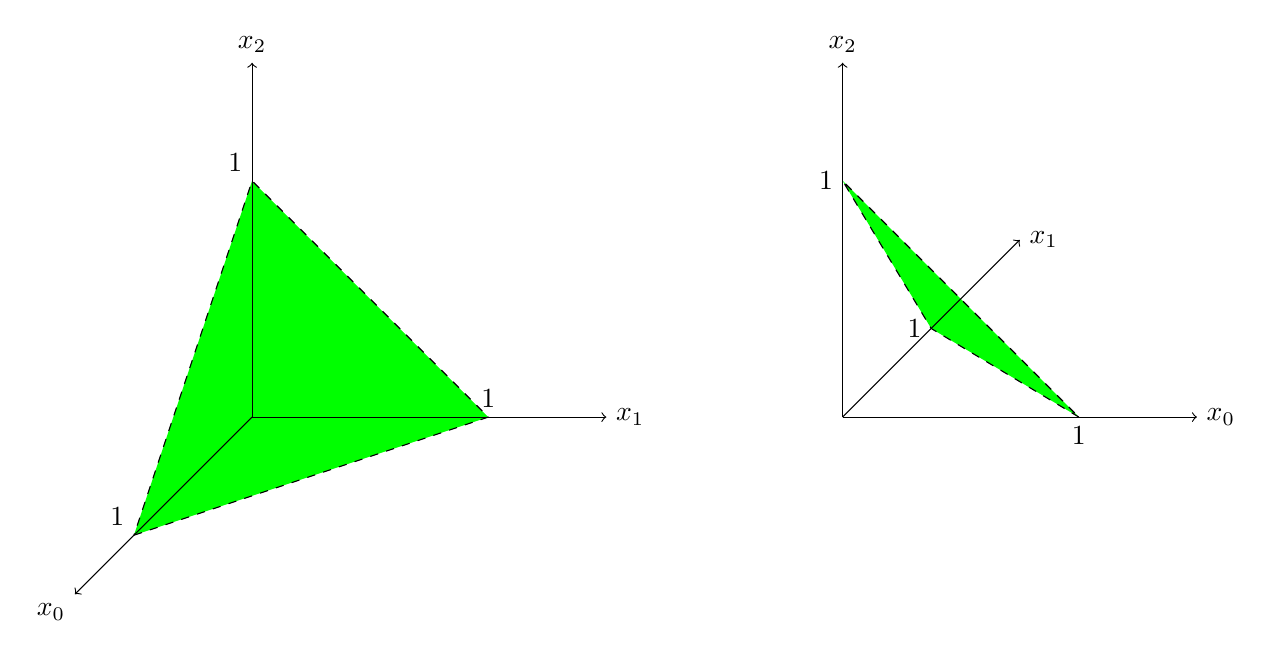
\begin{tikzpicture}[scale=0.75]
  %left
  \filldraw[dashed,fill=green]
    (-7,-2) node[above left] {$1$}
    --
    (-1,0) node[above] {$1$}
    --
    (-5,4) node[above left] {$1$}
    --
    cycle;
  \draw[->]
    (-5,0)
    --
    (-8,-3) node[below left] {$x_{0}$};
  \draw[->]
    (-5,0)
    --
    (1,0) node[right] {$x_{1}$};
  \draw[->]
    (-5,0)
    --
    (-5,6) node[above] {$x_{2}$};

  %right
  \filldraw[dashed,fill=green]
    (9,0) node[below] {$1$}
    --
    (6.5,1.5) node[left] {$1$}
    --
    (5,4) node[left] {$1$}
    --
    cycle;
  \draw[->]
    (5,0)
    --
    (11,0) node[right] {$x_{0}$};
  \draw[->]
    (5,0)
    --
    (8,3) node[right] {$x_{1}$};
  \draw[->]
    (5,0)
    --
    (5,6) node[above] {$x_{2}$};
\end{tikzpicture}
\caption{The standard simplex in dimension $0$ (top), $1$ (middle) and $2$ (bottom)}
\label{fig:stdsmplx}
\end{figure}
\\
The \textbf{face opposing $e_{i}$} in the $n$-dimensional standard simplex is - again as a subspace -
\begin{align*}
  \blacktriangle_{i}^{[n-1]}
  &:=
  \left\lbrace
      \sum_{j=0}^{n}
      x_{j}e_{j}
      \in
      \blacktriangle^{[n]}
    \colon
      x_{i}
      =
      0
  \right\rbrace
\end{align*}
It is obvious that there is a homeomorphism
\begin{align*}
  \delta_{i}^{n-1}
  \colon
  \blacktriangle^{[n-1]}
  &\to
  \blacktriangle_{i}^{[n-1]}
\end{align*}
and how it can be defined\footnote{keeping the ordering of the vertices}. We are now able to define \textbf{singular $n$-simplices} in a topological space $X$. These are just continuous maps
\begin{align*}
  \sigma
  \colon
  \blacktriangle^{[n]}
  &\to
  X
\end{align*}
and we let them be the elements of a set $S_{n}(X)$. To avoid case analysis we set $S_{n}(X) = \emptyset$ for $n < 0$. The set $S_{n}(X)$ can be turned into a free abelian group by the covariant functor $F$ assigning the set its free object
\begin{align*}
  C_{n}(X)
  &:=
  F(S_{n}(X))
\end{align*}
in $\mathbf{Ab}$. Next, for $\sigma \in S_{n}(X)$ define
\begin{align*}
  \partial_{n}(\sigma)
  &:=
  \sum_{i=0}^{n}
  (-1)^{i}
  \sigma
  \circ
  \delta_{i}^{n-1}
  \in
  C_{n-1}(X)
\end{align*}
Then $\partial_{n}$ can be (uniquely) extended to a morphism in $\mathbf{Ab}$, which is, for simplicity, again called $\partial_{n}$. It is straightforward to show that
\begin{align*}
  \partial_{n-1}
  \circ
  \partial_{n}
  &=
  0
\end{align*}
Hence $((C_{n}(X)),(\partial_{n}))$ is a chain complex. For a map $f \colon X_{1} \to X_{2}$ we define
\begin{align*}
  S_{n}(f)(\sigma)
  &:=
  f
  \circ
  \sigma
  \in S_{n}(X_{2})
\end{align*}
for $\sigma \in S_{n}(X_{1})$. Again, $S_{n}(f)$ can be (uniquiely) extended to a morphism $C_{n}(f) \colon C_{n}(X_{1}) \to C_{n}(X_{2})$ in $\mathbf{Ab}$. The idea developed here can be expanded to pairs of topological spaces, that is, elements $(X,A)$ of $\mathrm{ob}_{\mathbf{Top_{2}}}$ in the following way: set\footnote{note that if $A = \emptyset$ then $C_{n}(A)$ is trivial and thus $C_{n}((X,\emptyset))$ can be identified with $C_{n}(X)$}
\begin{align*}
  C_{n}((X,A))
  &:=
  C_{n}(X)
  /
  C_{n}(A)
\end{align*}
Since $\partial_{n}(C_{n}(A)) \subset C_{n-1}(A)$, a morphism
\begin{align*}
  \tilde{\partial}_{n}
  \colon
  C_{n}((X,A))
  &\to
  C_{n-1}((X,A))
  ,\quad
  [c]
  \mapsto
  [\partial_{n}c]
\end{align*}
in $\mathbf{Ab}$ is induced by $\partial_{n}$ which in abuse of notation is again called $\partial_{n}$. It is then immediate that $((C_{n}((X,A))),(\partial_{n}))$ is a chain complex. In a similiar vein
\begin{align*}
  C_{n}(f)
  &\colon
  C_{n}((X_{1},A_{1}))
  \to
  C_{n}((X_{2},A_{2}))
\end{align*}
is defined. Hence there is covariant functor $C$ from $\mathbf{Top_{2}}$ to $\mathbf{CC}$ which assigns to $(X,A)$ the chain complex $((C_{n}((X,A))),(\partial_{n}))$ and to $f \colon (X_{1},A_{1}) \to (X_{2},A_{2})$ the chain map $(C_{n}(f))$. The natural idea is to compose the functor $C$ with the homology group functors $H_{n}$ in order to get a homology theory. (HT2) is then immediate from the exact sequence of chain complexes
\begin{equation*}
\begin{tikzcd}[row sep=2.2em,column sep=2.6em]
  0
  \ar{r}
  &
  C((A,\emptyset))
  \ar{r}
  &
  C((X,\emptyset))
  \ar{r}
  &
  C((X,A))
  \ar{r}
  &
  0
\end{tikzcd}
\end{equation*}
The verification of the other axioms is a rather long story and therefore omitted here.\footnote{for brevity we have presented a {\glqq}Bourbaki-style{\grqq}-version of homology but actually (co)homology can be presented in a pretty intuitive way by considering CW-complexes as is done in \cite{8b5861fc}} Now singular cohomology is just the dualized version of singular homology with respect to some abelian group $G$, that is, $C$ becomes a contravariant functor $C^{\prime}$ by dualizing the constructed chain complex to a cochain complex and then $C^{\prime}$ is composed with $H^{n}$.
